Para o desenvolvimento do trabalho foram utilizados alguns componentes externos, tanto de \emph{hardware} quanto de \emph{software}. Foi utilizado o computador \emph{Raspberry Pi} e seu módulo de câmera, a linguagem de programação \emph{Python} e a biblioteca de visão computacional \emph{OpenCV} juntamente com outras bibliotecas auxiliares que permitam integrar o \emph{OpenCV} com a linguagem de programação \emph{Python} e o módulo de camera do \emph{Raspberry Pi}.

\section{Raspberry Pi}
\label{sec:raspi}

Raspberry Pi é um computador construído em uma placa de circuito do tamanho de um cartão de crédito desenvolvido pela Raspberry Pi Foundation\footnote{https://www.raspberrypi.org/}. Existem diversos modelos de Raspberry Pi no mercado, o utilizado no trabalho é um dos mais recentes, o Raspberry Pi 3 model B. Foi utilizado o sistema
operacional \emph{Raspbian}, que é o sistema operacional oficial suportado pela \emph{Raspberry Pi Foundation}.

\begin{figure}[H]
	\centering
	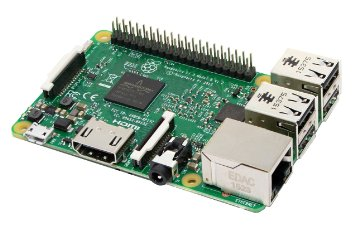
\includegraphics[width=88mm]{raspberrypi.jpg}
	\caption{O Raspberry Pi 3 model B}
	\label{fig:raspberrypi}
\end{figure}

O computador é limitado, pois tem um processador
quad-core ARMv8 de 1.2GHz e apenas 1GB de memória RAM\@. Pela limitação do
\emph{hardware} é possível que algumas aplicações fiquem mais lentas do que
ficariam em um computador mais potente, apesar disso, o Raspberry Pi é um
computador bem completo e capaz de exercer todas as funções de um computador
normal.

\section{OpenCV}
\label{sec:opencv}

OpenCV (\emph{Open Source Computer Vision Library}) é uma biblioteca \emph{open
source} de visão computacional e aprendizado de máquina. Contém mais de 2500
algoritmos otimizados nessas áreas, incluindo algoritmos clássicos e recentes. A biblioteca é escrita nativamente em C++, e dispõe de interfaces para C, C++,
Python, Java e MATLAB, suportando os sistemas operacionais Windows, Linux,
Android e Mac OS.\footnote{http://opencv.org/}

No desenvolvimento deste trabalho foi utilizada a linguagem de programação \emph{Python}. O motivo da escolha dessa linguagem se dá por ser uma linguagem muito usada para OpenCV\@, contendo muita documentação. Algumas outras bibliotecas são utilizadas para trabalhar com \emph{OpenCV} e \emph{Python}. A biblioteca \emph{numpy}\footnote{http://www.numpy.org/} é uma biblioteca de computação científica em \emph{Python}, que inclui funções de processamento numérico e vetores que são utilizados pelo \emph{OpenCV} para representar as imagens. 

Para as aplicações de aprendizado de máquina foi utilizada a biblioteca \emph{ml} que é um módulo do \emph{OpenCV}. Esta biblioteca contém um conjunto de classes e métodos para classificação estatística, regressão e agrupamento de dados.\footnote{http://docs.opencv.org/2.4/modules/ml/doc/ml.html}

Também foi utilizado o pacote \emph{picamera}\footnote{https://picamera.readthedocs.io/en/release-1.12/},
que possui uma interface em \emph{Python} para se comunicar com o módulo de camera do \emph{Raspberry Pi}.
É possível utilizar as funções próprias de captura de imagem da camera do \emph{OpenCV}, mas foi optado por utilizar o \emph{picamera}, por ser uma interface mais específica para a camera utilizada.

As escolhas de ferramentas e bibliotecas foram feitas
com objetivo de maximizar os resultados ao final do trabalho, para criar
um balanço entre facilidade de implementação e qualidade do reconhecimento.
